\section{Measure of the contact forces and torques}
In the previous sections the hybrid force-position control architecture was described
and the assumption was made that the wrench $\vec{w}_{S}$ (see eq. \ref{eq:joint_space_dyn})
that the environment exerts on the hand was available as a feedback signal.
\par
In this section it is explained how such a wrench can be obtained starting from the \emph{raw} signal
coming from a common force/torque sensor and what are the main problems encountered in doing that.

\subsection{Newton-Euler equations}
In order to understand what are the actual quantities measured by a force torque sensor it is useful
to describe, by means of the Newton-Euler approach, the motion of a rigid body, attached to the
sensor through a mounting plate, due to external forces and torques.
\begin{figure}[h]
  \centering
  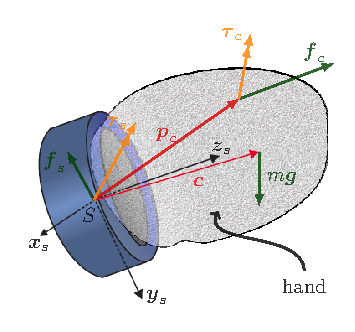
\includegraphics[scale=1.2]{ft_sensor_object}
  \caption{F/t sensor with hand attached \label{fig:ft_sensor_object}}
\end{figure}


The resulting equations are the following

\begin{equation}
  \prescript{s}{}{ \vec{f}}_{s} = -\prescript{s}{}{ \vec{f}}_{pl} -\prescript{s}{}{ \vec{f}}_{c} -m \prescript{s}{}{ \vec{g}}
  + m \prescript{s}{}{ \vec{a}}_{cm}
\end{equation}
\begin{equation}\label{eq:ne_torque_1}
  \begin{split}
  \prescript{s}{}{ \vec{\tau}}_{s} =& -\prescript{s}{}{ \vec{\tau}}_{pl} -\prescript{s}{}{ \vec{\tau}}_{c}
  - \prescript{s}{}{ \tilde{\vec{p}}}_{c} \prescript{s}{}{ \vec{f}}_{c}
  + \prescript{s}{}{ \tilde{\vec{g}}} m\prescript{s}{}{\vec{c}} \\
  & - \prescript{s}{}{ \tilde{\vec{a}}}_{cm} m \prescript{s}{}{ \vec{c}}
  + \prescript{s}{}{ I}_{cm} \prescript{s}{}{\vec{\alpha}}
  + \prescript{s}{}{ \tilde{\vec{\omega}}} \prescript{s}{}{ I}_{cm} \prescript{s}{}{ \vec{\omega}}\\
  \end{split}
\end{equation}
where
$\vec{f}_{s}$ and $\vec{\tau}_{s}$ are the forces and torques exerted by the sensor on the rigid body,
$\vec{f}_{pl}$ and $\vec{\tau}_{pl}$ are due to the mounting plate,
$\vec{f}_{c}$ and $\vec{\tau}_{c}$ are the \emph{external} forces and torques exerted on the rigid body in the interaction
with the environment,
$\vec{c}$ is the vector from the center of the sensor to the CoM of the rigid body,
$\vec{p}_{c}$ is the vector from the center of the sensor to the contact point with the environment,
$I_{cm}$ is the inertia matrix of the rigid body with respect to the CoM,
$\vec{g}$ is the gravity vector, $\vec{a}_{cm}$ is the linear acceleration of the CoM of the rigid body,
$\vec{\omega}$ is the angular velocity of the rigid body and
$\vec{\alpha}$ is the angular acceleration of the rigid body.
It should be noted that the wrench $\vec{w}_{S}$  is given by
\[
\vec{w}_{S} =
\begin{bmatrix}
  \vec{f}_{c}\\
  \vec{\tau}_{c} +\tilde{\vec{p}}_{c} \vec{f}_{c}\\
\end{bmatrix}
\]
\par
Since in this project the force/torque sensor is primarily used to control the contact force when the end-effector
is still or when it moves along straight lines the angular velocity and the angular acceleration of the end-effector
attached to the sensor can be neglected leading to the equations
\begin{equation}
  \label{eq:ne_force_2}
   \vec{f}_{s} = - \vec{f}_{pl} - \vec{f}_{c} -m  \vec{g} + m  \vec{a}_{cm}
\end{equation}
\begin{equation}
  \label{eq:ne_torque_2}
   \vec{\tau}_{s} = - \vec{\tau}_{pl} - \vec{\tau}_{c} - \tilde{\vec{p}}_{c}  \vec{f}_{c}
   + \tilde{\vec{g}} m\vec{c} -  \tilde{\vec{a}}_{cm} m  \vec{c}
\end{equation}

\subsection{Software induced offset}
The hardware of the force/torque sensor is built in a such way that the forces and torques exchanged
with the rigid body attached to it are measured. With reference to the equations (\ref{eq:ne_force_2})
and (\ref{eq:ne_torque_2}) the signal produced by the sensor can be written as

\[
\vec{f}_{m} = -\vec{f}_{s} + \vec{f}_{sw,off}
\]
\[
\vec{\tau}_{s} = -\vec{\tau}_{s} + \vec{\tau}_{sw,off}
\]
where $\vec{f}_{sw, off}$ and $\vec{\tau}_{sw,off}$ represent the offset introduced by
the sensor when the user activates the \emph{calibration} of the sensor. This operation
is performed when the sensor is \emph{still} and not in contact with the environment
and the resulting offset is chosen such that $\vec{f}_{m,0} = \vec{\tau}_{m,0} = \vec{0}$
where the zero subscript represents the calibration condition. Simple substitutions show that
\[
\vec{f}_{sw,off} = \vec{f}_{s,0} = -\vec{f}_{pl} -m \prescript{s}{}{ \vec{g}}_{0}
\]
\[
\vec{\tau}_{sw,off} = \vec{\tau}_{s,0} = -\vec{\tau}_{pl} + \prescript{s}{}{ \tilde{\vec{g}}}_{0} m\vec{c}
\]
where $\vec{g}_{0}$ is the value assumed by the gravity expressed in the sensor frame $S$ at the
moment of the calibration.
\par
Taking into account the expressions of the offset the measured forces and torques in absence of angular
motions can be written as
\begin{equation}
  \label{eq:m_force_2}
  \vec{f}_{m} = \vec{f}_{c} +m \vec{g} -m \prescript{s}{}{ \vec{g}}_{0} - m  \vec{a}_{cm}
\end{equation}
\begin{equation}
  \label{eq:m_torque_2}
  \vec{\tau}_{m} = \vec{\tau}_{c} + \tilde{\vec{p}}_{c}  \vec{f}_{c}
  - \tilde{\vec{g}} m\vec{c} + \prescript{s}{}{ \tilde{\vec{g}}}_{0} m\vec{c} +  \tilde{\vec{a}}_{cm} m  \vec{c}
\end{equation}
As suggested by the previous formulas in order to obtain the part of the measure related to the contact
with the environment it is required to estimate the mass of the rigid body $m$, the position of the centre of
mass with respect to center of the sensor $\vec{c}$ and the offsets $-m \prescript{s}{}{ \vec{g}}_{0}$
and $\prescript{s}{}{ \tilde{\vec{g}}}_{0} m\vec{c}$.
The gravity $\prescript{s}{}{ \vec{g}}$ expressed in sensor frame can be obtained using the direct kinematics software facilities
developed for the project while the linear acceleration $\vec{a}_{cm}$ can be obtained using an appropriate
jacobian, its derivative and an estimate of the angular velocities and accelerations of the joints
of the robot.

\subsection{Estimation of parameters and offsets}
Since all the quantities to be estimated are revealed even when the sensor is still
it is possible to estimate them by acquiring a certain number of measures each when
the robot, hence the sensor, assumes a static pose. The estimation can be obtained
from the measures using a \emph{linear} least squares approach since there exist
a linear relationship between the measurements and the parameters

\[
\begin{split}
  \begin{bmatrix}
    \vec{f}_{m} \\
    \vec{\tau}_{m} \\
  \end{bmatrix} &=
  \begin{bmatrix}
    \vec{g} m + (-m \prescript{s}{}{ \vec{g}}_{0}) \\
    -\tilde{\vec{g}} m\vec{c} + (\prescript{s}{}{ \tilde{\vec{g}}}_{0} m\vec{c}) \\
  \end{bmatrix}\\
  & =
  \begin{bmatrix}
    \vec{g} & 0_{3 \times 3} & I_{3x3} & 0_{3x3} \\
    \vec{0} & -\tilde{\vec{g}} & 0_{3x3} & I_{3x3}
  \end{bmatrix}
  \begin{bmatrix}
    m \\
    m \vec{c} \\
    -m \prescript{s}{}{ \vec{g}}_{0} \\
    \prescript{s}{}{ \tilde{\vec{g}}}_{0} m\vec{c} \\
  \end{bmatrix}\\
  &=
  H(\prescript{s}{}{ \vec{g}}) \vec{\theta}
\end{split}
\]
where $\prescript{s}{}{ \vec{g}} = \prescript{s}{}{ \vec{g(\vec{q})}}$ depends on the configuration $\vec{q}$ of the robot.
\par
Given n configurations of the robot the estimate is given by
\[
\begin{split}
  \hat{\vec{\theta}} &=
  \begin{bmatrix}
    H(\vec{q}^{1})\\
    \vdots \\
    H(\vec{q}^{n})\\
  \end{bmatrix}^{+}
  \begin{bmatrix}
    \vec{f}_{m}^{1} \\
    \vec{\tau}_{m}^{1} \\
    \vdots \\
    \vec{f}_{m}^{n} \\
    \vec{\tau}_{m}^{n} \\
  \end{bmatrix}
  =
  H_n^{+}
  \begin{bmatrix}
    \vec{f}_{m}^{1} \\
    \vec{\tau}_{m}^{1} \\
    \vdots \\
    \vec{f}_{m}^{n} \\
    \vec{\tau}_{m}^{n} \\
  \end{bmatrix}\\
\end{split}
\]
where it can be shown that for $n \ge 3$ the matrix $H_n$ is always full column rank
so that $H_n^{+} = H_n(H_n^{T} H_n)^{-1}$.
Once the estimate is computed contact forces and torques can be evaluted as
\[
\hat{\vec{f}}_c = \vec{f}_m - \hat{\theta}_{1} \vec{g} - \hat{\vec{\theta}}_{5:7} + \hat{\theta}_{1} \hat{\vec{a}}_{cm}(\vec{q},\vec{\dot{q}},\vec{\ddot{q}})
\]
\[
\hat{\vec{\tau}}_c + \tilde{\vec{p}}_c  \hat{\vec{f}}_c = \vec{\tau}_m + \tilde{\vec{g}} \hat{\vec{\theta}}_{2:4} - \hat{\vec{\theta}}_{8:10} - \tilde{\hat{\vec{a}}}_{cm}(\vec{q},\vec{\dot{q}},\vec{\ddot{q}}) \hat{\vec{\theta}}_{2:4}
\]
where $\hat{\vec{a}}_{cm}$ is an estimate of the linear acceleration of the centre of mass of the rigid body.
\subsubsection{Example of estimation}
An example of estimation, with $n=60$, is shown in the figures below where each step represents a new row of the
matrix $H_{60}$. The estimated parameters are the following:
\begin{itemize}
\item $\hat{m} = \SI{0.6848}{kg}$ (see Fig. \ref{fig:mass_estimation})
\item $\hat{\vec{c}} =
  \begin{bmatrix}
    0.32 & 0.28 & 11.20
  \end{bmatrix}^T$ cm  (see Fig. \ref{fig:com_estimation})
\item $-\hat{m} \prescript{s}{}{ \hat{\vec{g}}}_{0} =
  \begin{bmatrix}
    0.8577 & -6.0316 & 0.8438 
  \end{bmatrix}^T
  $N  (see Fig. \ref{fig:off_f_estimation})
\item $\prescript{s}{}{ \tilde{\hat{\vec{g}}}}_{0} \hat{m}\hat{\vec{c}} =
  \begin{bmatrix}
    0.8299 & 0.0772 & -0.0149  
  \end{bmatrix}^T
  $Nm  (see Fig. \ref{fig:off_t_estimation})
\end{itemize}
\begin{table}[h]
  \begin{tabular}{cc}
    \begin{subfigure}{0.5\textwidth}
      \centering
      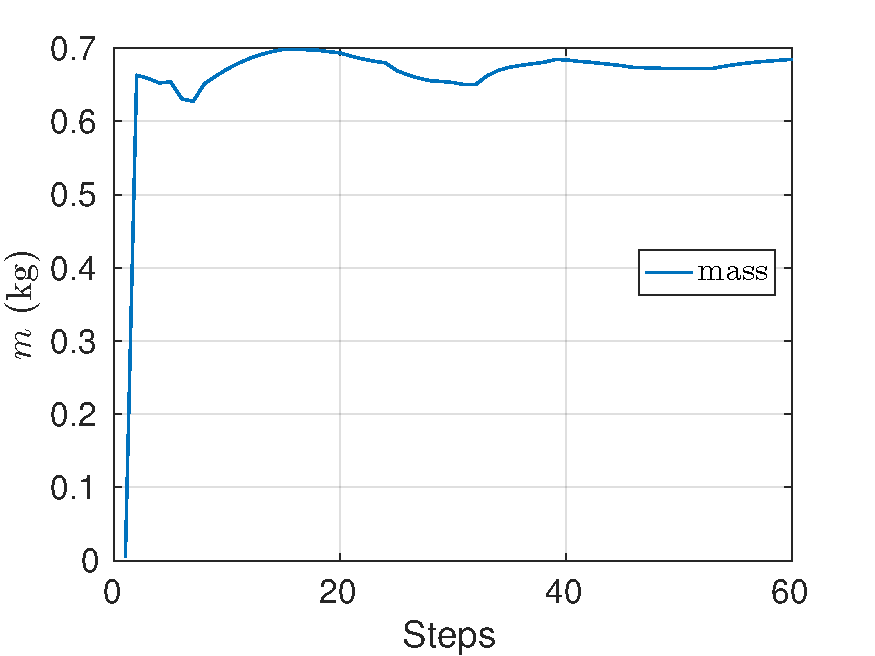
\includegraphics[scale=0.5]{mass}
      \caption{Mass estimation \label{fig:mass_estimation}}
    \end{subfigure}&
    \begin{subfigure}{0.5\textwidth}
      \centering
      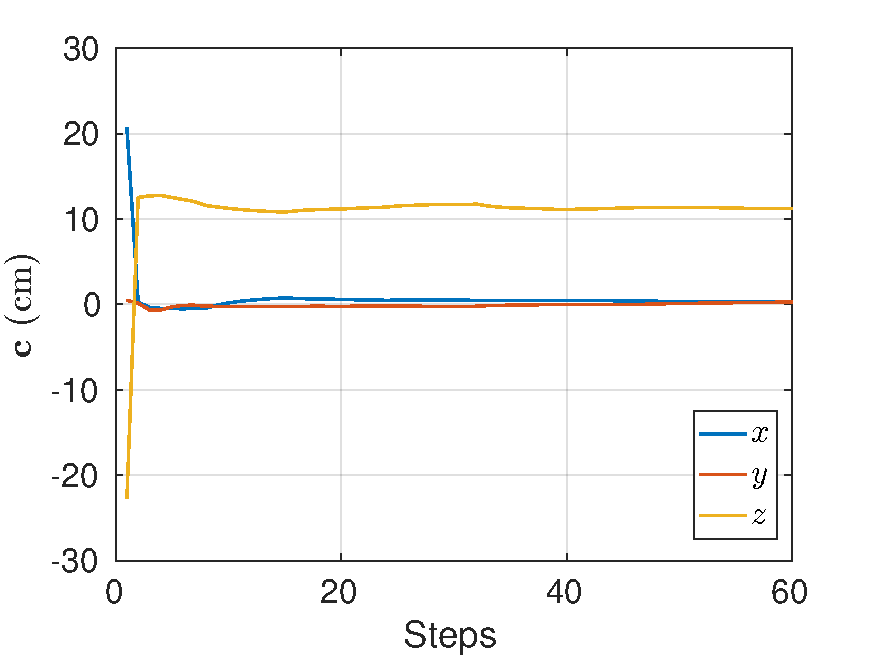
\includegraphics[scale=0.5]{com}
      \caption{CoM estimation\label{fig:com_estimation}}
    \end{subfigure}
  \end{tabular}
  \caption{Estimation results}
\end{table}
It can be verified that
\[
\frac{||\hat{m}\hat{\vec{g}}_0||}{9.81} = 0.6270 \approx 0.6848 = \hat{m}
\]
as expected.
\begin{table}[h]
  \begin{tabular}{cc}
    \begin{subfigure}{0.5\textwidth}
      \centering
      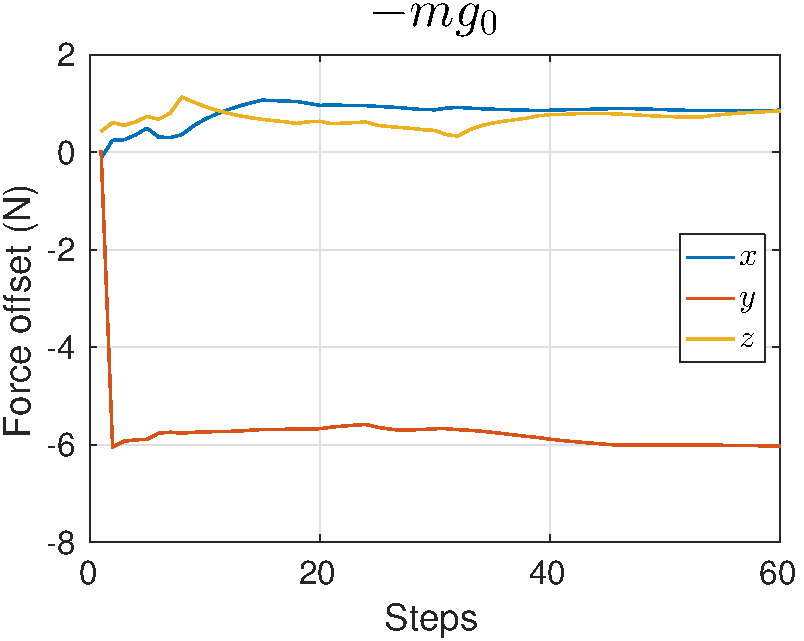
\includegraphics[scale=0.5]{off_f}
      \caption{Offset estimation (Force) \label{fig:off_f_estimation}}
    \end{subfigure}&
    \begin{subfigure}{0.5\textwidth}
      \centering
      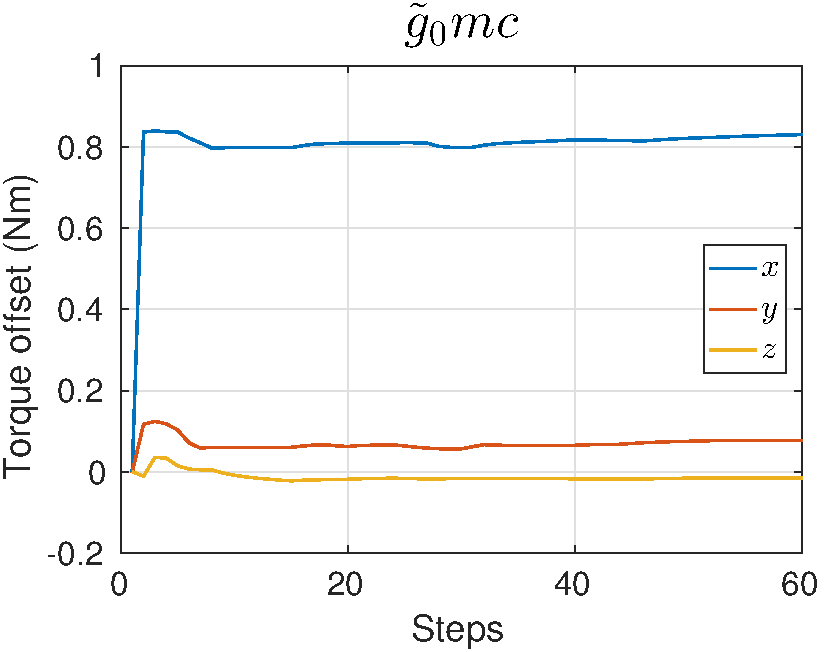
\includegraphics[scale=0.5]{off_t}
      \caption{Offset estimation (Torque) \label{fig:off_t_estimation}}
    \end{subfigure}
  \end{tabular}
  \caption{Estimation results}
\end{table}
\newpage
